\chapter{Unsupervised Learning}
\textbf{Unsupervised learning} is a type of machine learning in which the algorithm is not provided with any pre-assigned labels or scores for the training data. As a resut, unsupervised learning algorithms must first self-discover any naturally occurring patterns in that training data set.

In unsupervised learning we observe data that are sampled from an unknown distribution \(p_{\text{data}} \in \Delta(\mathcal{X})\), but we lack observations about the target variables (e.g. we don't have access to class labels). It is still possible to detect some pattern to grab some information from this data, we can compensate for the lack of this features by designing an appropriate objective function. 

\section{Tasks in depth}
In particular the objective function we have designed will lead us to solve three families of problems:
\begin{itemize}[topsep={0pt}, partopsep={0pt}]
    \itemsep0pt
    \item Dimensionality reduction;
    \item Clustering;
    \item Density estimation.
\end{itemize}
\subsection{Dimensionality Reduction}
The \textbf{dimensionality reduction} is the transformation of data from a high-dimensional space into a low-dimensional space so that the low-dimensional space representation retains some meaningful properties of the original data, ideally close to its intrinsic dimension.

The task of the dimensionality reduction is to find a function \(f \in \mathcal{Y}^{\mathcal{X}}\) mapping each high-dimensional input \(x \in \mathcal{X}\) to a lower dimensional, embedding \(f(x) \in \mathcal{Y}\), where \(dim(\mathcal{Y}) \ll dim(\mathcal{X})\).

The purposes of dimensionality reduction are to compress the input data by reducing the feature dimensionality, while preserving as much information as possible. The way information loss is measured yields different algorithms. This reduces time of subsequent data elaboration and/or storage. Furthermore, it enables better visualization of data and reduces the curse of dimensionality.

\begin{figure}[h!]
    \centering
    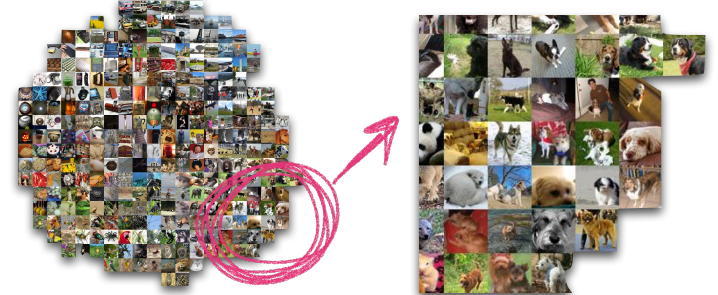
\includegraphics[width=.5\textwidth]{066}
    \caption{Dimensionality reduction.}
    \label{fig:066}
\end{figure}

\subsection{Clustering}
\textbf{Clustering} is the task of grouping a set of objects in the same group (called a cluster) are more similar to each other than to those in other groups. 

The appropriate clustering algorithm and parameter settings (including parameters such as the distance function to use, a density threshold or the number of expected clusters) depend on the individual data set and intended use of the results. Cluster analysis as such is not an automatic task, but an iterative process of knowledge discovery or interactive multi-objective optimization that involves trial and failure. It is often necessary to modify data preprocessing and model parameters until the result achieves the desired properties.

The task of clustering is to find a function \(f \in \mathbb{N}^{\mathcal{X}}\) that assigns each input \(x \in \mathcal{X}\) a cluster index \(f(x) \in \mathcal{N}\). All points mapped to the same index form a cluster.

Clustering is used because it allows to analyze data by grouping together data points that exhibit some regular pattern or similarity under some predefined criterion. It can be used to compress data by reducing the number of data points as opposed to reducing the feature dimensionality.

\begin{figure}[h!]
    \centering
    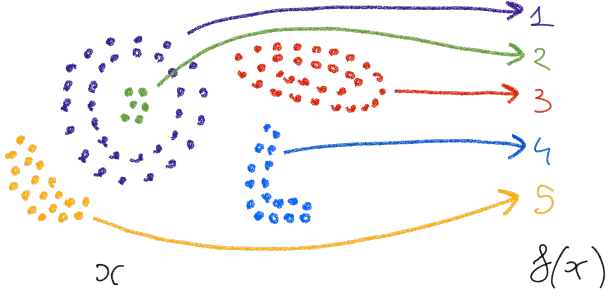
\includegraphics[width=.5\textwidth]{065}
    \caption{Clustering.}
    \label{fig:065}
\end{figure}

Applications example of clustering are: cluster users by reference (e.g. based on movie ratings), group genes families from gene sequences, find communities in social networks, etc.

\subsection{Density Estimation}
The \textbf{density estimation} is the construction of an estimate, based on observed ata, of an unobservable underlying probability density function. 

A very natural use of density estimates is in the informal investigation of the properties of a given set of data. Density estimates can give valuable indication of such features as skewness and multimodality in the data. In some cases they will yield conclusions that may then be regarded as self-evidently true, while in others all they will do is to point the way to further analysis and/or data collection.

The task of density estimation is to find a probability distribution \(f \in \Delta(\mathcal{X})\) that fits the data \(x \in \mathcal{X}\).

\begin{figure}[h!]
    \centering
    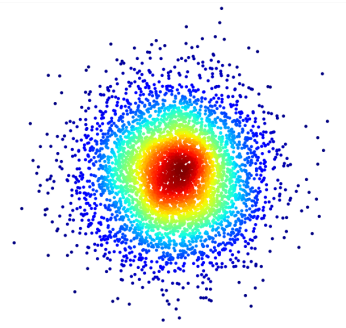
\includegraphics[width=.5\textwidth]{067}
    \caption{Density estimation.}
    \label{fig:067}
\end{figure}

Density estimation allows to get an explicit etimate of the unknown probability distribution that generated the training data. It enables the generation of new data by sampling from the estimated distribution, and it enables the detection of anomalies/novelties in terms of data points that a exhibit low probabilities according to the estimated distribution.

\section{Principal Component Analysis}
The \textbf{principal components} of a collection of points in a real coordinate space are a sequence of \(p\) unit vectors, where the \(i\)-th vector is the direction of a line that best fits the data while being orthogonal to the first \(i-1\) vectors. Here, a best-fitting line is defined as one that minimizes the average squared distance from the points to the line. These directions constitute an orthonormal basis in which different individual dimensions of the data are linearly uncorrelated.

\textbf{Principal Component Analysis (PCA)} is the process of computing the principal components and using them to perform a change of basis on the data, sometimes using only the first few principal compoents and ignoring the rest --- namely, drop dimensions of least variance.

\begin{figure}[t!]
    \centering
    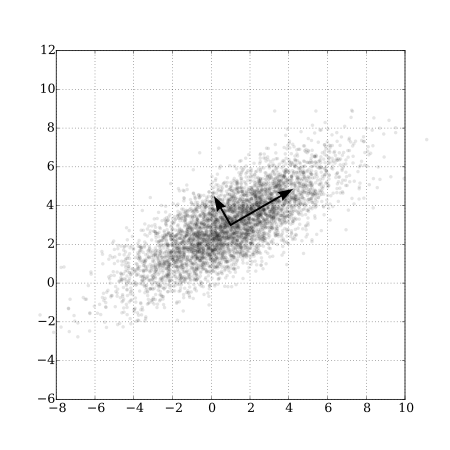
\includegraphics[width=.5\textwidth]{068}
    \caption{PCA of a multivariate Gaussian distribution centered at \((1,3)\).}
    \label{fig:068}
\end{figure}

\begin{wrapfigure}{l}{0.35\textwidth}
    \begin{center}
        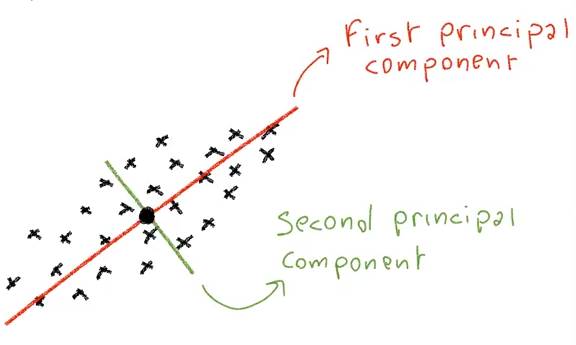
\includegraphics[width=0.35\textwidth]{069}
        \caption{}
    \end{center}
    \label{fig:069}
\end{wrapfigure}
In a nutshell, we have a set of data points that are represented by black crosses symbols in Figure~\ref{fig:069}. We want to find the direction that explains the maximum variance of the data, in this case is the direction indicated by the red line --- that is our principal component. Our second principal component is orthogonal to the first principal component.

When we found our components, now the directions lead us to a new coordinate system. The way PCA allows us to do dimensionality reduction is by dropping the dimennsions of least variance.
\begin{figure}[h!]
    \centering
    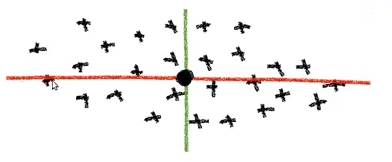
\includegraphics[width=.5\textwidth]{070}
    \caption{}
    \label{fig:070}
\end{figure}

\subsection{Variance Along Unit Direction}
We are interested in computing the variance with the constraint that our parameter vector \(w\) has norm 1, this means: \(\vec{w}^T\vec{w} = ||\vec{w}|| = 1\). 

So what we do is to take each data point \(\vec{x}_i\), and project \(\vec{x}_i\) to another line that corresponds to the direction of our weight vector \(w\). To do that we use an auxiliary point \(\vec{c}\), and we compute the distance between \(\vec{x}_i\) and \(\vec{c}\), then \(t_i = (\vec{x}_i - \vec{c})^T \vec{w}\).

Once we defined our reference point \(\vec{c}\) we are interested in maximizing the variance of the data points. To do that we first have to compute expected value of \(t\) considering all the \(t_i\) of all the data points \(\vec{x}_i\) in our dataset.
\begin{equation}
    \mathbb{E}\left[t\right] = \frac 1 n \sum_{i=1}^n t_i = \frac 1 n \sum_{i=1}^n (\vec{x}_i - \vec{c})^T \vec{w} = \bar{\vec{x}}^T \vec{w} - \vec{c}^T \vec{w}
\end{equation}
Where \(\bar{\vec{x}} = \frac 1 n \sum_i x_i\) is the mean, now we can compute the variance:
\begin{align}
    \mathbb{V}ar\left[t\right] &= \frac 1 n \sum_{i=1}^n \left(t_i - \mathbb{E}[t]\right)^2 = \frac 1 n \sum_{i=1}^n \left[(\vec{x}_i - \bar{\vec{x}})^T \vec{w}\right]^2\\
    & = \frac 1 n \sum_{i=1}^n \left(\bar{\vec{x}}_i^T \vec{w}\right)^2 = \vec{w}^T \left[ \frac 1 n \bar{X}\bar{X}^T \right] \vec{w} = \vec{w}^T C \vec{w}
\end{align}
where \(t_i = (\vec{x}_i - \vec{c})^T \vec{w}\), \(\bar{X} = [\bar{\vec{x}}_1, \bar{\vec{x}}_2, ..., \bar{\vec{x}}_n]\), and \(C = \left[ \frac 1 n \bar{X}\bar{X}^T \right]\) is the covariance matrix.

\subsection{Eigenvalue Decomposition}
Let \(A \in \mathbb{R}^{m \times m}\), symmetric. There exists \(U = \left[ \vec{u}_1, \vec{u}_2, ..., \vec{u}_m \right] \in \mathbb{R}^{m \times m}\) and \(\vec{\lambda} = (\lambda_1, \lambda_2, ..., \lambda_m)^T \in \mathbb{R}^{m}\) such that:
\begin{equation}
    A = U \Lambda U^T = \sum_{j=1}^m \lambda_j \vec{u}_j \vec{u}_j^T \qquad \text{and} \qquad U^T U = UU^T = I
\end{equation}
where \(U\) is the matrix of the eigenvectors, \(\Lambda\) is a square matrix with values all 0 except of the principal diagonal, that is composed by \(\lambda_1, \lambda_2, ..., \lambda_m\), \(I\) is the identity matrix, \(\vec{u}_j\) is an eigenvector and \(\lambda_j\) is the corresponding eigenvalue. 

Note that we assume descending ordering \(\lambda_1 \geq \lambda_2 \geq ... \geq \lambda_n\).

\subsubsection{First Principal Component}
\begin{equation}
    \vec{w}_1 \in \arg \max \left\{ \vec{w}^T C \vec{w} : \vec{w}^T \vec{w} = 1 \right\}
\end{equation}
The largest eigenvalue of \(C\) is the variance along the first principal component, and the first principal component \(\vec{w}_1\) is the corresponding eigenvector.

\paragraph{Proof}
By eigenvale decomposition \(C = \sum_j \lambda_j \vec{u}_j \vec{u}_j^T\) and assume eigenvalue sorted in descending order, i.e. \(\lambda_1 \geq \lambda_2 \geq ... \geq \lambda_m\). Then, \(\vec{w}_1^T C \vec{w}_1 = \sum_j \lambda_j (\vec{w}_1^T \vec{u}_j)^2 \leq \lambda_1\) because
\begin{equation*}
    \sum_j (\vec{w}_1^T \vec{u}_j)^2 = \vec{w}_1^T \sum_j \vec{u}_j \vec{u}_j^T \vec{w}_1 = \vec{w}_1^T UU^T \vec{w}_1 = \vec{w}_1^T \vec{w}_1 = 1
\end{equation*}
It follows that \(\lambda_1 \geq \vec{w}_1^T C \vec{w}_1 \geq \vec{u}_1^T C \vec{u}_1 = \lambda_1\) which implies that 
\begin{equation*}
    \vec{w}_1^T C \vec{w}_1 = \vec{u}_1^T C \vec{u}_1
\end{equation*}
Therefore \(\vec{u}_1\) i.e. the eigenvector corresponding to the largest eigenvalue \(\lambda_1\) of \(C\), is a first principal component and \(\lambda_1\) the variance along it.

\subsubsection{Second Principal Component}
\begin{equation}
    \vec{w}_2 \in \arg \max \left\{ \vec{w}^T C \vec{w} : \vec{w}^T \vec{w} = 1, \vec{w} \perp \vec{w}_1 \right\}
\end{equation}
The largest eigenvalue of \(C\) is the variance along the second principal component, and the second principal component \(\vec{w}_2\) is the corresponding eigenvector.

\paragraph{Proof}
By eigenvale decomposition \(C = \sum_j \lambda_j \vec{u}_j \vec{u}_j^T\) and assume eigenvalue sorted in descending order, i.e. \(\lambda_1 \geq \lambda_2 \geq ... \geq \lambda_m\). Then, \(\vec{w}_2^T C \vec{w}_2 = \sum_{j=1}^m \lambda_j (\vec{w}_2^T \vec{u}_j)^2 = \lambda_1 \vec{w}_2^T \vec{u}_1 + \sum_{j=2}^m \lambda_j (\vec{w}_2^T \vec{u}_j)^2 \leq \lambda_2\) because
\begin{equation*}
    \sum_j (\vec{w}_2^T \vec{u}_j)^2 = \vec{w}_2^T \sum_j \vec{u}_j \vec{u}_j^T \vec{w}_2 = \vec{w}_2^T UU^T \vec{w}_2 = \vec{w}_2^T \vec{w}_2 = 1
\end{equation*}
It follows that \(\lambda_2 \geq \vec{w}_2^T C \vec{w}_2 \geq \vec{u}_2^T C \vec{u}_2 = \lambda_2\) which implies that 
\begin{equation*}
    \vec{w}_2^T C \vec{w}_2 = \vec{u}_2^T C \vec{u}_2
\end{equation*}
Therefore \(\vec{u}_2\) i.e. the eigenvector corresponding to the second largest eigenvalue \(\lambda_2\) of \(C\), is a second principal component and \(\lambda_2\) the variance along it.

\subsubsection{\(i\)-th Principal Component}
\begin{equation}
    \vec{w}_i \in \arg \max \left\{ \vec{w}^T C \vec{w} : \vec{w}^T \vec{w} = 1, \vec{w} \perp \vec{w}_j \text{ for } 1 \leq j < i\vec{} \right\}
\end{equation}
The \(i\)-th largest eigenvalue of \(C\) is the variance along the \(i\)-th principal component. The \(i\)-th principal component \(\vec{w}_i\) is the corresponding eigenvector.

The proof is similar to the one we already saw.

\subsection{PCA using Eigenvalue Decomosition}
To summarize, we can provide the algorithm that allows us to compute the principal components through eigenvalue decomposition.

Given data points \(X = \left[\vec{x}_1, \vec{x}_2, ..., \vec{x}_n \right]\), we apply some centering \(\bar{X} = X - \frac 1 n X 1_n 1_n^T\), where \(1_n\) is a vector of ones, so we take our data points vector and subtract the centres (mean) of the data points. Ones we have the center, we compute the covariance matrix \(C = \frac 1 n \bar{X} \bar{X}^T\), and then we can compute the eigenvalue decomposition \(U\), \(\lambda = eig(C)\). Our principal components will be \(W = U = \left[ \vec{u}_1, \vec{u}_2, ..., \vec{u}_m \right]\), with variances \(\lambda = \left( \lambda_1, \lambda_2, ..., \lambda_m \right)\).
\begin{algorithm}
    \caption{PCA using ED}
    \KwData{$X=\left[x_1,x_2,\ldots,n_n\right]$}
    $\bar X = X - \frac 1 n X 1_n 1_n^T$\;
    $C = \frac 1 n \bar X \bar X^T$\;
    $U$, $\lambda = $ eig$(C)$\;
    \Return{Principal components $W=U=[u_1,u_2,\ldots,u_m]$ and variances $\lambda = (\lambda_1, \lambda_2, \ldots, \lambda_m)$}
\end{algorithm}

\subsection{PCA Using Singular Value Decomposition (SVD)}
\subsubsection{Singular Value Decomposition}
Let \(A \in \mathbb{R}^{m \times n}\). There exist \(U \in \mathbb{R}^{m \times k}, s \in \mathbb{R}^k\) with \(s_1 \geq s_2 \geq ... \geq s_k > 0\) and \(V \in \mathbb{R}^{n \times k}\) such that:
\begin{equation}
    A = USV^T \qquad \text{ and } \qquad U^TU ? V^TV = I
\end{equation}

\subsubsection{PCA with SVD}
In order to use PCA, we have to compute SVD of \(\bar{X}: U, \vec{s}, V = SVD(\bar{X})\). The principal components are \(U = \left[ \vec{u}_1, \vec{u}_2, ..., \vec{u}_m \right]\), and the variances are \(\left( \frac {s_1^2} n, \frac {s_2^2} n, ...,  \frac {s_k^2} n \right)\). This because \(\bar{X} = USV^T\), and \(C = \frac 1 n \bar{X} \bar{X}^T = \frac 1 n USV^T VSU^T = U \frac {s^2} n U^T\), where \(\frac {s^2} n\) corresponds to \(\Lambda\) in the case of the eigenvalue decomposition.
\begin{algorithm}
    \caption{PCA using SVD}
    \KwData{$X=\left[x_1,x_2,\ldots,n_n\right]$}
    $\bar X = X - \frac 1 n X 1_n 1_n^T$\;
    $U$, $s$, $V = $ SVD$(\bar X)$\;
    \Return{Principal components $W=U=[u_1,u_2,\ldots,u_k]$ and variances $\lambda = \left( \frac {s_1^2} n, \frac {s_2^2} n, \ldots, \frac {s_k^2} n \right)$}
\end{algorithm}
\subsection{Dimensionality Reduction Using PCA}
\begin{wrapfigure}{l}{0.35\textwidth}
    \begin{center}
        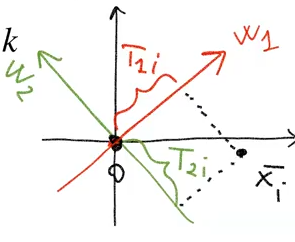
\includegraphics[width=0.35\textwidth]{071}
        \caption{}
    \end{center}
    \label{fig:071}
\end{wrapfigure}
Now we discuss how it is possible to reduce dimensionality using PCA. Let's consider \(\hat{W} = \left[\vec{w}_1, \vec{w}_2, ..., \vec{w}_k \right]\) hold the first \(k\) principal components derived from data points \(\bar{X} = \left[\bar{\vec{X}}_1, \bar{\vec{X}}_2, ..., \bar{\vec{X}}_n \right]\).

If we compute
\begin{equation}
    T = \hat{W}^T \bar{X} \in \mathbb{R}^{k \times n}
\end{equation}
it will induce a change of the coordinate system with respect to the \(k\) principal components in \(\hat{W}^T\), and this will reduce the dimension of the features to \(k\) if we have chosen the first \(k\) principal components.

We can use eigenvalue decomposition or SVD algorithms that avoid computing the full decomosition.

\subsection{Alternative Interpretation}
There is also an alternative interpretation of the first princiapl component analysis: principal components can be interpreted as the line in the space with minimal squared distance from the data points. A similar interpretation can be given to the other principal components.

\begin{figure}[h!]
    \centering
    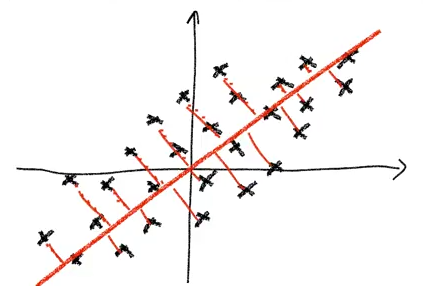
\includegraphics[width=.5\textwidth]{072}
    \caption{Alternative interpretation of the principal components.}
    \label{fig:072}
\end{figure}

Note that the \textbf{scale of the feature dimensions} matter when we are using PCA, so if the features are expressed in different units, it is recommended to normalize and scale them to have unit standard deviation. 

How many princiapl components should we choose? The number depends on the goal and on the application. In general we have no way to know a-priori how many components do we need, unless we are in the context of supervised classification methods, this means that first we are applying PCA and reducing the dimensions of our data points and then we can apply some classification method.

Nonetheless we can compute the cumulative proportion of explained variance, which for the first \(k\) principal components is given by:
\begin{equation}
    \text{Eigenvalue decomposition: } \frac {\sum_{j=1}^k \lambda_j} {\sum_{j=1}^m C_{jj}} \qquad \text{SVD: } \frac {\sum_{j=1}^k s_j^2} {\sum_{ij} \bar{X}_{ji}^2}
\end{equation}
this allows to estimate the amount of information loss

\subsection{Kernel PCA}
PCA reduces the dimensionality via a linear transformation. By using the kernel trick one can apply PCA in a higher dimensional space, yielding a non-linear transformation in the original space.

\begin{figure}[h!]
    \centering
    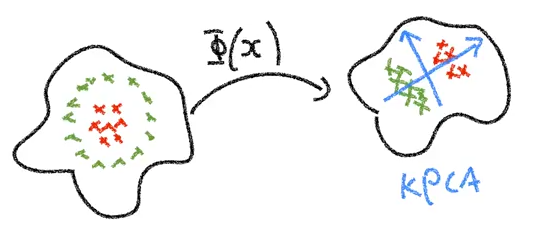
\includegraphics[width=.5\textwidth]{073}
    \caption{Kernel PCA.}
    \label{fig:073}
\end{figure}

\section{\(k\)-Means Clustering}
Given data points \(X = \left[ \vec{x}_1, \vec{x}_2, ..., \vec{x}_n \right] \in \mathbb{R}^{d \times n} \), and \(k\) a fixed number of clusters. Our goal is to fina a partition of data points into \(k\) sets \(\mathcal{C}_1, \mathcal{C}_2, ..., \mathcal{C}_k\) minimizing the variation \(V(\mathcal{C}_j)\) within each set \(V(\mathcal{C}_j)\):
\begin{equation}
    \min_{\mathcal{C}_1, ..., \mathcal{C}_k} \sum_{j=1}^k V(\mathcal{C}_j)
\end{equation}
The variation is typically given by the euclidean distance \(V(\mathcal{C}_j) = \sum_{i \in \mathcal{C}_j} || \vec{x}_i - \vec{\mu}_j ||^2\) where \(\vec{\mu}_j = \frac 1 {|\mathcal{C}_j|} \sum_{i \in \mathcal{C}_j} \vec{x}_i\) is the centroid of \(\mathcal{C}_j\).

\subsection{Optimization Algorithm}
The algorithm that is used to minimize the objective function is an iterative algorithm that is very simple. We first initialize the assignment and we assign randomly each data point to one cluster, in particular we initialize the centroid of each cluster and then we will iterate the following steps while clusters change:
\begin{enumerate}
    \item Compute cluster centroids \(\vec{\mu}_1, ..., \vec{\mu}_k\);
    \item Assign each data point to the closest centroid forming a new cluster, i.e.
    \begin{equation}
        \mathcal{C}_j = \left\{ i \in \{1, ..., n\} : j = \arg \min_\mathcal{C} || \vec{x}_i - \vec{\mu}_\mathcal{C} || \right\}
    \end{equation}
\end{enumerate}

\begin{algorithm}
    \caption{$k$-means}
    Use some initialization strategy to get some initial cluster centroids $\mu_1,\ldots,\mu_k$\;
    \While{clusters change}{
        Assign each datapoint to the closest centroid forming new clusters\;
        $\mathcal C_j = \{i \in \{1,\ldots,n\} : j = \arg \min_l ||\vec x_i - \mathcal \mu_l\}$\;
        Compute the cluster centroids $\mu_1,\ldots,\mu_k$\;
    }
\end{algorithm}

\subsection{Properties}
The algorithm is guaranteed to converge, because it strictly improves the objective if there is at least a cluster change and the set of possible partitions is finite. It is not guaranteed to find the global minimum but a local one. the problem is NP-hard even on the plane (\(d=2\)). 

Furthermore, it is sensitive to the scale o features. Features normalization is required in case of features with different scales.

\newpage
\begin{exercise}
    \ex What is dimensionality reduction?
    \ex Describe the clustering.
    \ex Describe the density estimation.
    \ex What is Principal Component Analysis?
    \ex Describe the PCA using the eigenvalue decomposition.
    \ex Describe the PCA using the singular value decomposition.
    \ex How can we use PCA for dimensionality reduction?
    \ex Describe the \(k\)-means clustering.
    \ex What are the properties of the \(k\)-means clustering?
\end{exercise}